\documentclass[]{ximera}
%handout:  for handout version with no solutions or instructor notes
%handout,instructornotes:  for instructor version with just problems and notes, no solutions
%noinstructornotes:  shows only problem and solutions

%% handout
%% space
%% newpage
%% numbers
%% nooutcomes

%I added the commands here so that I would't have to keep looking them up
%\newcommand{\RR}{\mathbb R}
%\renewcommand{\d}{\,d}
%\newcommand{\dd}[2][]{\frac{d #1}{d #2}}
%\renewcommand{\l}{\ell}
%\newcommand{\ddx}{\frac{d}{dx}}
%\everymath{\displaystyle}
%\newcommand{\dfn}{\textbf}
%\newcommand{\eval}[1]{\bigg[ #1 \bigg]}

%\begin{image}
%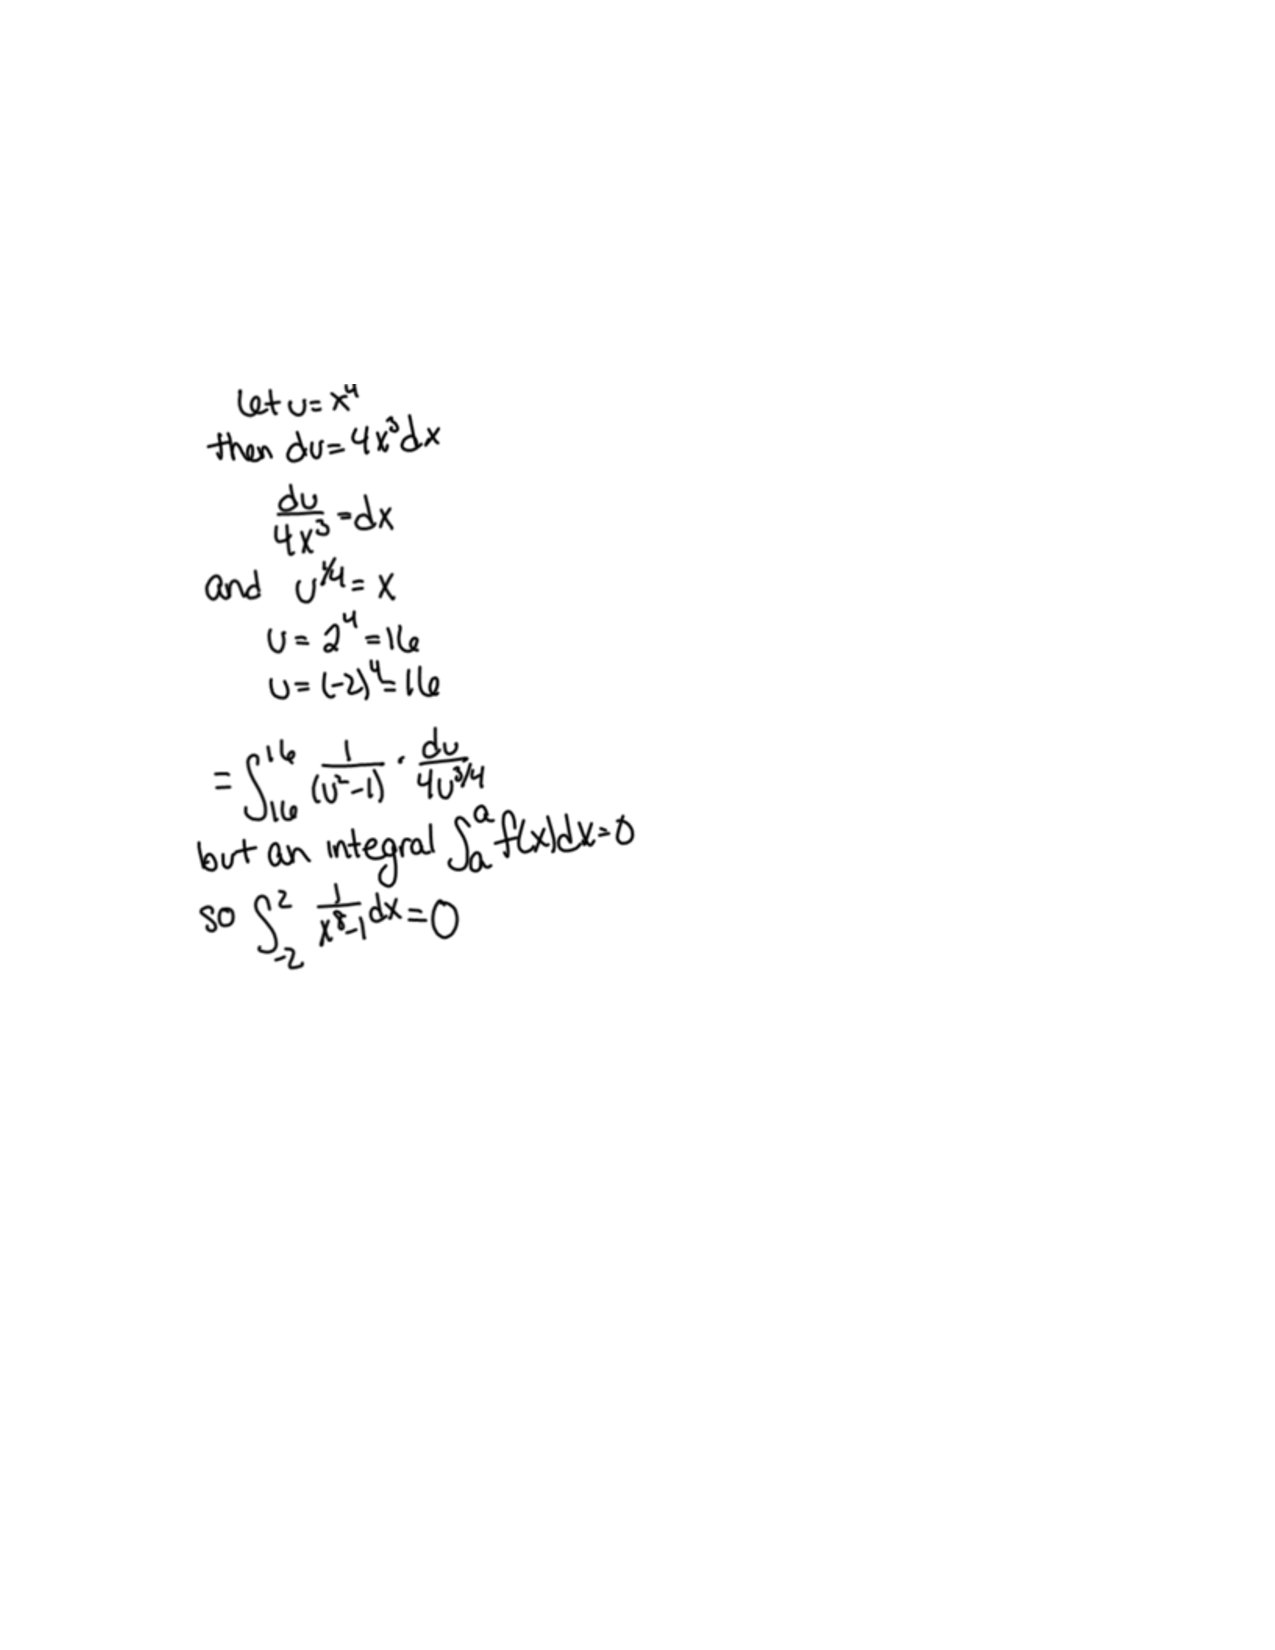
\includegraphics[trim= 170 420 250 180]{Figure1.pdf}
%\end{image}

%add a ``.'' below when used in a specific directory.
\newcommand{\RR}{\mathbb R}
\renewcommand{\d}{\,d}
\newcommand{\dd}[2][]{\frac{d #1}{d #2}}
\renewcommand{\l}{\ell}
\newcommand{\ddx}{\frac{d}{dx}}
\newcommand{\dfn}{\textbf}
\newcommand{\eval}[1]{\bigg[ #1 \bigg]}

\usepackage{multicol}

\renewenvironment{freeResponse}{
\ifhandout\setbox0\vbox\bgroup\else
\begin{trivlist}\item[\hskip \labelsep\bfseries Solution:\hspace{2ex}]
\fi}
{\ifhandout\egroup\else
\end{trivlist}
\fi} %% we can turn off input when making a master document

\title{Trigonometric integrals}  

\begin{document}
\begin{abstract}		\end{abstract}
\maketitle



\begin{comment}
\section{Warm up:}

	\begin{freeResponse}
	
	\end{freeResponse}
	
\begin{instructorNotes}

\end{instructorNotes}
\end{comment}







\section{Group work:}



%problem 1
\begin{problem}
Evaluate the following integrals
	\begin{enumerate}
	
	\item  $\int \tan^{23} x \sec^6 x \d x$
	\begin{freeResponse}
		\begin{align*}
		\int \tan^{23} x \sec^6 x \d x 
		&= \int \tan^{23} x \sec^4 x \sec^2 x \d x  \\
		&= \int \tan^{23} x \left( 1 + \tan^2 x \right)^2 \sec^2 x \d x .
		\end{align*}
	We now substitute
		{\color{red}
		\[
		u = \tan x 	\qquad	\Longrightarrow		\qquad	\d u = \sec^2 x \d x.
		\]
		}
	Then
		\begin{align*}
		\int \tan^{23} x \left( 1 + \tan^2 x \right)^2 \sec^2 x \d x
		&= \int u^{23} (1+u^2)^2 \d u  \\
		&= \int u^{23} (1 + 2u^2 + u^4) \d u  \\
		&= \int \left( u^{23} + 2u^{25} + u^{27} \right) \d u  \\
		&= \frac{1}{24} u^{24} + \frac{1}{13} u^{26} + \frac{1}{28} u^{28} + C  \\
		&= \frac{1}{24} \tan^{24} x + \frac{1}{13} \tan^{26} x + \frac{1}{28} \tan^{28} x + C.
		\end{align*}
	\end{freeResponse}
	
	
	
	\item  $\int \tan^2 x \sec x \d x$ \qquad {\color{red} Hint:  $\int \sec x \d x = \ln | \sec x \tan x| + C$}
	\begin{freeResponse}
		\begin{align}
		\int \tan^2 x \sec x \d x
		&= \int \left( \sec^2 x - 1 \right) \sec x \d x  \nonumber	\\
		&= \int \sec^3 x \d x - \int \sec x \d x  		\nonumber	\\
		&= \int \sec^3 x \d x - \ln | \sec x \tan x| 	\qquad	{\color{red}\text{from the hint}}	\label{equation 1}
		\end{align}
	Now, in an attempt to evaluate $\int \sec^3 x \d x$, we use integration by parts with
		{\color{red}
		\[
		u = \sec x 				\qquad	\d v = \sec^2 x \d x
		\]
		\[
		\d u = \sec x \tan x \d x	\qquad	v = \tan x.
		\]
		}
	So
		\begin{equation}\label{equation 2}
		\int \sec^3 x \d x = \sec x \tan x - \int \tan^2 x \sec x \d x.
		\end{equation}
	Combining equations \eqref{equation 1} and \eqref{equation 2} yields
		\begin{align*}
		\int \tan^2 x \sec x \d x &= \int \sec^3 x \d x - \ln | \sec x \tan x|   \\
		\int \tan^2 x \sec x \d x &= \sec x \tan x - \int \tan^2 x \sec x \d x - \ln | \sec x \tan x |  \\
		2 \int \tan^2 x \sec x \d x &= \sec x \tan x - \ln | \sec x \tan x | + C  \\
		\int \tan^2 x \sec x \d x &= \frac{1}{2} \left( \sec x \tan x - \ln | \sec x \tan x | \right) + C.
		\end{align*}
	\end{freeResponse}
	
	
	
	\item  $\int \tan^2 x \sin x \d x$
	\begin{freeResponse}
		\begin{align*}
		\int \tan^2 x \sin x \d x
		&= \int \frac{\sin^2 x}{\cos^2 x} \sin x \d x  \\
		&= \int \frac{1-\cos^2 x}{\cos^2 x} \sin x \d x.
		\end{align*}
	Now we substitute
		{\color{red}
		\[
		u = \cos x 		\qquad	\Longrightarrow		\qquad	\d u = - \sin x \d x, \quad - \d u = \sin x \d x.
		\]
		}
	This gives us that
		\begin{align*}
		\int \tan^2 x \sin x \d x
		&= \int \frac{1-u^2}{u^2} (-1) \d u  \\
		&= \int \frac{u^2 - 1}{u^2} \d u  \\
		&= \int \left( 1 - u^{-2} \right) \d u  \\
		&= u + \frac{1}{u} + C  \\
		&= \cos x + \sec x + C.
		\end{align*}
	\end{freeResponse}
	
	\end{enumerate}
	
\end{problem}

\begin{instructorNotes}
All three parts involve standard strategies learned in the online lessons.  
For each, split the problems between the groups.  
Then discuss each problem as a class, getting input from the group(s) that worked on that problem.
\end{instructorNotes}







%problem 2
\begin{problem}
Evaluate
	\[
	\int_{- \pi}^0 \sqrt{1 - \cos^2 x} \d x.
	\]
	\begin{freeResponse}
		\begin{align*}
		\int_{- \pi}^0 \sqrt{1 - \cos^2 x} \d x
		&= \int_{- \pi}^0 \sqrt{\sin^2 x} \d x  \\
		&= \int_{- \pi}^0 | \sin x | \d x.
		\end{align*}
	Now, when $-\pi \leq x \leq 0$, $\sin x \leq 0$.  
	Thus, on this region, $|\sin x | = - \sin x$.
	So we continue
		\begin{align*}
		\int_{- \pi}^0 \sqrt{1 - \cos^2 x} \d x
		&= \int_{- \pi}^0 - \sin x \d x  \\
		&= \eval{\cos x}_{-\pi}^0  \\
		&= \cos(0) - \cos(-\pi) = 1 - (-1) = 2.
		\end{align*}
	\end{freeResponse}
		
\end{problem}

\begin{instructorNotes}
You may want to do this problem as a whole class - perhaps play-acting by claiming that it is equal to $\int_{-\pi}^0 \sin x \d x$ rather than $\int_{-\pi}^0 \left| \sin x \right|  \d x$
\end{instructorNotes}







\begin{comment}
%problem 3
\begin{problem}

	\begin{freeResponse}
	
	\end{freeResponse}

\end{problem}

\begin{instructorNotes}

\end{instructorNotes}
\end{comment}
















	
	
	
	
	
	
	
	
	

	










								
				
				
	














\end{document} 


















